\documentclass[preprint]{aastex} 

\usepackage[top=1in, bottom=1in, left=1in, right=1in]{geometry}
\usepackage{amsmath}
\usepackage{graphicx}
\usepackage{mdwlist}
\usepackage{natbib}
\usepackage{natbibspacing}
\setlength{\bibspacing}{0pt}
\setlength{\parskip}{0pt}
\setlength{\parsep}{0pt}
\setlength{\headsep}{0pt}
\setlength{\topskip}{0pt}
\setlength{\topmargin}{0pt}
\setlength{\topsep}{0pt}
\setlength{\partopsep}{0pt}
\setlength{\footnotesep}{8pt}
\pagestyle{empty}
\citestyle{aa}

%Project Description (8-pages maximum), including the following:
%- A statement of which of the four categories of MSIP is most appropriate
%for this proposal as the first sentence (see section II. Program Description).
%- A scientific justification. For Open Access Capabilities, explain the
%uniqueness and lack of general availability of the capability.
%- A description of the broader impacts, including student training.
%- A description of benefits to the community (observing time, data products, etc.)
%- An outline of the project management plan (where appropriate).
%Note: Results from Prior NSF Support should not be included. Links to URLs may
%not be used.

\begin{document}
\title{Hydrogen Epoch of Reionization Arrays (HERA): Beyond Detection}
% A statement of which of the four categories of MSIP is most appropriate
%for this proposal as the first sentence (see section II. Program Description).

This proposal targets the Mid-Scale Science Projects category of the 
Mid-Scale Innovations Program solicitation.
The Hydrogen Epoch of Reionization Arrays (HERA) is a program for using the
unique capabilities of the 21cm hyperfine line to trace neutral hydrogen
through the cosmic dawn of our Universe.  The HERA roadmap that was submitted
to the {\it New Worlds, New Horizons of Astronomy and Astrophysics} 2010
decadal survey, (hereafter NWNH) was given ``top priority in this [Radio,
Millimeter, and Sub-millimeter] category of recommended new facilities for
mid-scale funding." The HERA roadmap proceeded in three stages: HERA-IB called
for \$25M to complete the PAPER and MWA experiments; HERA-II budgeted \$62M for
an array with 0.1 km$^2$ of collecting area capable of characterizing the power
spectrum of cosmic reionization in detail; HERA-III targeted 1 km$^2$ of
collecting area to image reionization structures in detail.

The PAPER and MWA experiments are now fully constructed, and nearing the
completion of their groundbreaking science program over the coming two years.
Although significantly less than \$25M was invested in HERA-IA/B, these
`spearhead projects' are leading the global effort to tap the transformative
potential of the 21cm line as a probe of cosmic history.
The most difficult challenge involves balancing stringent sensitivity requirements 
against the need to suppress
foregrounds that are five orders of magnitude brighter than the signal.   In
this area, there has been a major breakthrough.  Based on a new understanding
of how instrumental characteristics can be leveraged to isolate foreground
emission from the cosmological signal on the basis of spectral smoothness,
foreground emission has been suppressed by four orders of magnitude in PAPER
observations, down to the current limits of PAPER's sensitivity.  HERA-IA/B instruments
are now sensitivity-limited, and making the first statistical detection of 21cm
reionization remains viable at the limits of the sensitivity of current
projects.

Given this new conclusive answer to the question of how to optimize 21cm reionization
experiments for foreground removal,
the time is ripe to launch the next phase of HERA.  We propose a
staged approach to building the next-generation experiment that incorporates these
new breakthroughs, targets reionization science beyond the first detection, and
is timed to begin producing transformative science just as current HERA-I instruments
are finishing.  As described below, recent technical breakthroughs favor
larger, close-packed antenna elements, and this has substantially altered the
HERA plan.  The next step for HERA targeted in this proposal delivers the 0.1
km$^2$ collecting area and associated science of HERA-II, but with less than
600 antennas, the budget (\$16.3M), project complexity, and project team are of
a modest HERA-IB scope.

\vspace{-0.25in}
\section{Scientific Justification}

The period beginning with the birth of the first luminous objects in the
universe, and culminating with the ionization of the intergalactic medium (IGM)
$\sim$500 Myrs later, is one of the last unexplored phases of cosmic evolution.
Exploring this epoch of reionization was highlighted as one of the three
``priority science objectives chosen by the [NWNH] survey committee for the
decade 2012-2021" \citep{astro2010}. Observations of Gunn-Peterson absorption
by the IGM toward the most distant quasars \citep{fan_et_al2006}, kinetic
Sunyaev-Zel'dovich features in the CMB \citep{zahn_et_al2012}, and CMB
anisotropy and polarization \citep{page_et_al2007,planck_et_al2013} indicate
that reionization was a complex process, starting perhaps as early as 
$z\approx14$, with the last vestiges of the the neutral IGM being etched away by
$z\approx6$.  Unfortunately, these ground-breaking results are limited in
diagnostic capabilities: the Gunn-Peterson effect saturates for even low
neutral fractions, and the CMB only provides an integral measure of the
Thompson optical depth back to recombination.

Redshifted emission from the 21cm hyperfine transition of neutral hydrogen has
gained considerable attention as a unique (albeit weak) tracer of the
primordial IGM.  The direct observation of the neutral IGM via this signal
would be an achievement comparable with the discovery of the CMB.  As
emphasized in NWNH \citep{astro2010}: ``The panel concluded that to explore the
discovery area of the epoch of reionization, it is most important to develop
new capabilities to observe redshifted 21-cm HI emission, building on the
legacy of current projects and increasing sensitivity and spatial resolution to
characterize the topology of the gas at reionization."

\begin{figure}[!ht]\centering
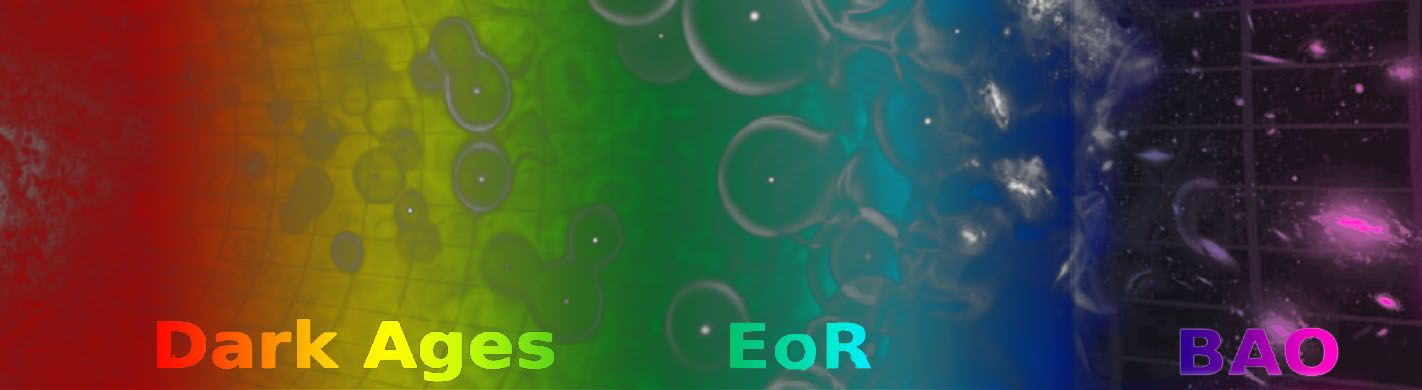
\includegraphics[width=6in]{plots/21cm_cosmo.jpg}
\caption{\small
The 21cm hyperfine line of neutral hydrogen represents the next frontier in
precision cosmology. Following recombination (left edge), the spin temperature
of 21cm emission is sensitive to the density and temperature of the
intergalactic medium (IGM) through the Dark Ages, evolves with the heating and
ionization of the IGM during the Epoch of Reionization (EoR), and
traces the distribution of galaxies as the universe expands,
leading up the the present day (right edge).  Color indicates
redshift, which stretches the 21cm line to frequencies ranging from 50 MHz
(red) to 1.4 GHz (violet).
}\label{fig:21cm_cosmo}
\end{figure}

The challenges associated with 21cm cosmology experiments are daunting.  Such
experiments require unprecedented levels of sensitivity, instrumental
calibration, and foreground characterization.  The spectral response of these
instruments is of paramount importance; it is used both for constructing the
line-of-sight direction of 3D space, and also for differentiating
smooth-spectrum foreground emission from spatial fluctuations in the
cosmological signal. The brightness temperatures of foregrounds, in the form of
galactic synchrotron emission, continuum point-sources, and polarized
galactic/extra-galactic emission, exceed the fluctuations of the 21cm signal by
more than 5 orders of magnitude
\citep{santos_et_al2005,pritchard_loeb2012,pober_et_al2013b}.

As is being discovered, these foregrounds are proving very difficult to attack
head-on.  To achieve the necessary sensitivity, experiments are driven toward
using interferometers, but the frequency dependence of the angular wavemode
sampled by an interferometer causes smooth-spectrum foregrounds to appear
unsmooth, degrading the separation that can be achieved between foregrounds and
$k$-modes of the 21cm power spectrum $\Delta^2_{21}(k)$.  
%XXX maybe remove jargon here and describe consensus of community around “the wedge”.
Experimental approaches adopted by LOFAR and the MWA aim to achieve sufficient
accuracy in foreground characterization and instrument calibration to model and
remove such chromatic effects.  However, this is proving to be an extremely
challenging and costly task, and it remains uncertain whether this approach is
practically viable given realistic limitations on calibration accuracy.

\begin{figure}[!ht]\centering
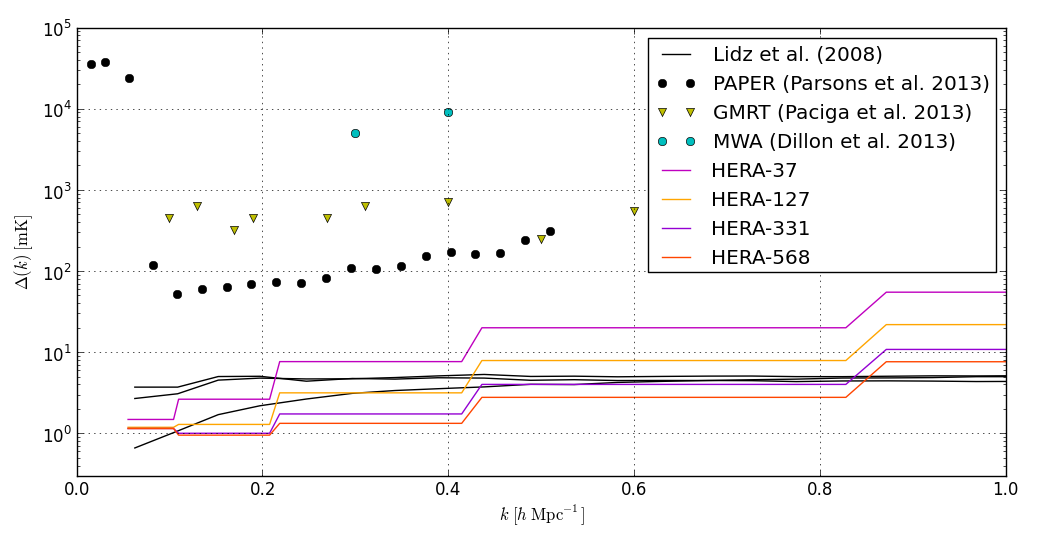
\includegraphics[height=3.0in]{plots/eor_pspec.png}
\caption{\small
Current best upper limits on the power spectrum of 21cm emission from
reionzation at $z=7.7$, made with a 32-antenna deployment of the PAPER
experiment \citep{parsons_et_al2013}. Black indicates the final measurements
with 2$\sigma$ confidence intervals. The yellow triangles indicate the previous
best 2$\sigma$ upper limits at $z=8.6$ \citep{paciga_et_al2013}. Magenta
illustrates a fiducial 50\% ionization model \citep{lidz_et_al2008}. The 8
orders of magnitude (in mK$^2$) of foreground suppression outside of the dashed
lines (left panel) are a testament to the crucial role that instrument design
plays in mitigating foreground systematics.
}\label{fig:eor_pspec}
\end{figure}

PAPER has made significant progress following a different approach.  Based on a
``delay-spectrum'' understanding of the mechanism for how instrumental
responses modulate foregrounds on spectral scales of cosmological interest
\citep{parsons_et_al2012b}, PAPER has optimized its instrument to focus on
regions in Fourier space that have weak coupling to foregrounds. XXX describe
optimization to foreshadow changes in HERA.  These regions are determined both
by chromatic instrumental responses and by the inherent frequency evolution of
the foregrounds.  As shown in Figure \ref{fig:eor_pspec}, observations based on
this new approach are demonstrating that the extremely stringent level of
foreground removal needed to access the 21cm signal is largely in hand, with
upper limits that are beginning to rule out cold reionization scenarios. 

\vspace{-0.25in}
\section{Project Description}

\begin{figure}[!ht]\centering
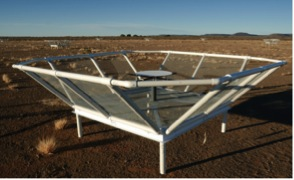
\includegraphics[height=1.75in]{plots/paper_element.jpg}
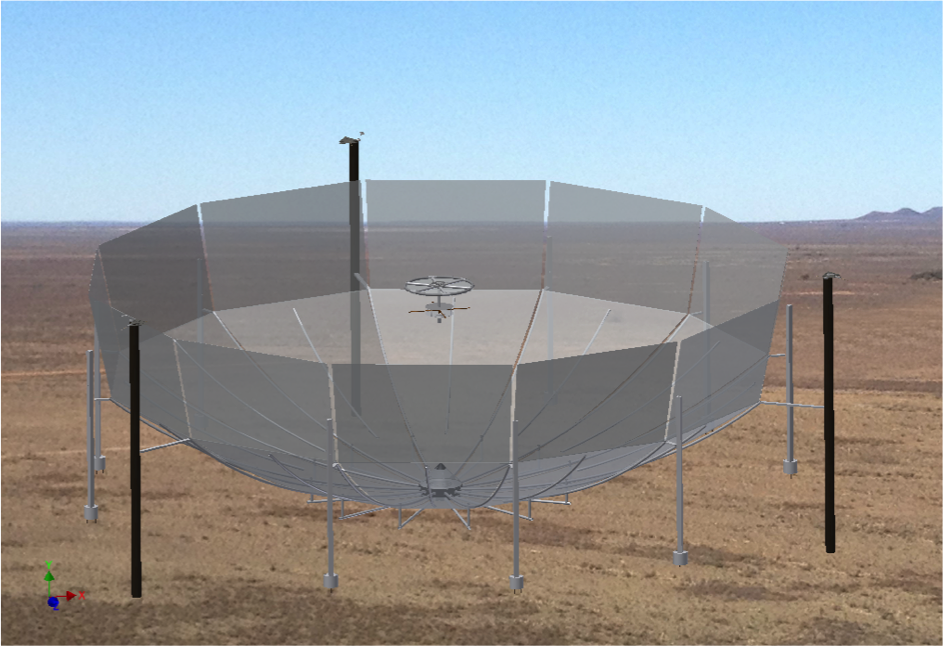
\includegraphics[height=1.75in]{plots/hera_dish.png}
\caption{\small
The PAPER element (left) provides a clean instrumental response as a function
of frequency \citep{parsons_et_al2010,parsons_et_al2012b}, which is crucial to
the foreground isolation shown in Figure \ref{fig:eor_pspec}.  A 14m dish
designed around the same feed (right) dramatically improves sensitivity while
constraining the path length and amplitude of
reflections to ensure that foreground isolation is not substantially degraded.  
}\label{fig:hera_dish}
\end{figure}

This HERA proposal targets a 568-element array that incorporates these proven
foreground avoidance techniques while addressing the sensitivity limitations of
current experiments.  With a better understanding of how antenna size and
separation affect the interaction of sensitivity and foreground isolation, it
has become clear that larger, close-packed antenna elements can yield up to 30
times the sensitivity of current elements without substantially degrading
foreground isolation.  Where PAPER’s elements lack collecting area and are
smaller than strictly required for foreground isolation, and the majority of
MWA and LOFAR elements are spaced too widely to avoid foregrounds, HERA employs
an extremely compact array of large --- but not {\it too} large --- antenna
elements, building on PAPER's design.  As illustrated in Figure
\ref{fig:hera_dish}, these elements consist of PAPER-style dipole feeds
suspended over 14m parabolic dishes.  The short ($\sim$5m) focal height of these
dishes is central to limiting the path length of reflections whose time-delay
gives rise to chromatic instrumental systematics. 

The size of the new HERA dish optimizes cost for a fixed sensitivity and level
of foreground isolation.  The associated reduction in the number of antenna
elements, combined with the fact that these dishes have no moving parts, are
built from inexpensive materials, and follow a simple construction that can be
delegated to local contractors, makes the cost of building HERA's Phase-II
experiment several times cheaper than was anticipated in the HERA roadmap
submitted to NWNH.  
%XXX talk a bit more about build-ability.

HERA follows a staged build-out plan similar to that championed by PAPER.  In
each deployment stage, improvements are incorporated into the system, and new
science capabilities are unlocked.  This approach has the advantage of
providing early access to science, permitting longer development times for
certain system components, and reducing the project risk by testing systems
early and changing them incrementally.  As shown in Figure \ref{fig:eor_pspec}, each
stage of HERA brings an associated improvement in sensitivity that allow key
aspects of 21cm reionization science to be addressed.  The timeline of HERA
development, along with the associated science producets, is outlined below. 

{\bf Year 1 (FY 2015)}.  In the first year, development of
infrastructure (ground leveling, power, basic network connectivity) begins
immediately on a new `K3' site approximately 10 km from the current PAPER site
at the Karoo Radio Observatory in South Africa.  As final PAPER-128
observations complete in Apr. 2015, the existing PAPER-128 antennas,
correlator, and EMC container are migrated to the K3 site, where they are
combined with 37 prototype HERA dishes that use existing PAPER feeds and
electronics, and are arranged in a compact hexagonal configuration.  Physical
construction is handled by students, engineers, and local interns.  Activities
for developing and improving HERA baluns, receivers, and feeds from PAPER
designs begin, as do the in-situ antenna calibration subsystems and the
longer-term development activities for node electronics, the (exploratory)
spatial FFT correlator, and the various software analysis pipelines.

{\bf Year 2 (FY 2016)}.  Commissioning observations begin with HERA-37,
correlated along with 91 PAPER elements using the PAPER correlator on site.
This first observations test the performance of the HERA dishes, verifying beam
patterns against known PAPER beam responses, and checking for any problematic
spectral structure arising from signal reflections.  Science observations begin
in Oct. 2015 and run until Apr. 2016.  Because HERA-37 has $\sim$10 times the sensitivity of
PAPER-128, thes observations have a high probability of
detecting the peak levels of the 21cm EoR power spectrum.   Development of site
infrastructure (high-bandwidth optical network, surveying, trenching) finishes.
Development activities begun in Year 1 continue, culminating in the
finalization and fabrication of improved HERA feeds and receivers in Jan.
2016.  As observations with HERA-37 complete, deployment of the next stage of
HERA begins: a larger, 127-element array of HERA dishes in a hexagonal
configuration, featuring new feeds and (if necessary) a refined dish design.
If possible, the 37 existing elements are retrofitted, but if necessary,
HERA-127 budgets for replacement.  Physical construction (trenching, pole
installation, assembly) is handled by local contractors.

{\bf Year 3 (FY 2017)}.  Construction of HERA-127 completes, and
science observations begin in Oct. 2016, again using the PAPER correlator.
Science papers from HERA-37 are published.   Node and correlator designs are
finalized and fabrication begins.  Science observations with HERA-127 complete
in Apr. 2017; analysis begins on a dataset capable of constraining the timing
and duration of reionization.  Deployment of HERA-331 begins.  Contractors lead
physical construction, expanding from the existing 127 elements.  Node
electronics are installed for all 331 elements, and a new, 331-element
GPU-based correlator is installed in the Karoo Array Processing Building
(KAPB), operating on digital data that are transmitted from the nodes through
optical links.  Additional data storage infrastructure is installed in the
KAPB.  The UPenn data analysis cluster is upgraded. 

{\bf Year 4 (FY 2018)}.  Construction of HERA-331 completes, and
science observations begin in Oct. 2017.   HERA-127 results are published.
Fabrication of nodes and antenna parts continues.  Science observations with
HERA-331 complete in Apr. 2018, and analysis begins on a dataset capable of
characterizing the slope of the power spectrum, distinguishing between various
sources of ionizing photons.  Deployment of HERA-568 begins, following the same
pattern as in Year 3.  If the design of the spatial FFT correlator is mature
and successfully tested in commissioning observations, the FX correlator
hardware will be repurposed as a spatial FFT correlator, with spare hardware
used to compute the real-time calibration parameters that are necessary to the
functioning of the spatial FFT correlator.

{\bf Year 5 (FY 2019)}.  In the final year, construction of HERA-568
completes, and science observations begin in Oct. 2018.  Papers from HERA-331
are published.  With build-out complete, all attention is now directed toward
preparing and testing final imaging and power-spectrum software pipelines, such
that processing proceeds on HERA-568 as data are available.  Science papers
resulting from these observations are published, including extensions of
analysis to lower frequency bands and imaging of bright reionization
structures.

%\section{Broader Impacts and Benefit to the Community}

%\section{Project Management Plan}

%\begin{table}
%\label{tab:params}
%\begin{tabular}{|l|rl|l|}
%\hline
%Parameter & Value & Units & Description \\
%\hline
%$N$  &  576  & & Number of Antennas \\
%$d$ & 14 & m & Antenna Diameter \\
%$f/d$ & 0.32 &  & Focal Length (fractional) \\
%$\Omega_{\rm P}$ & 0.026 & sr & Field of View (power) \\
%$\Omega_{\rm PP}$ & 0.013 & sr & Field of View (power$^2$) \\
%$\Omega_{\rm eff}$ & 0.052 & sr & Field of View (sensitivity) \\
%$B_{\rm samp}$ & 0--250 & MHz & Sampled Frequency Range \\
%$B_{\rm corr}$ & 100 & MHz & Correlated Bandwidth \\
%Config.	& 24 $\times$ 24 & & Square Grid Antenna Configuration\\
%$f/f_0$ & $1.5\cdot10^5$ & & Redundancy Metric (Parsons et al. 2012a) \\
%$A$ & 0.09 & km$^2$ & Total Collecting Area \\
%$\theta$ & 15 & arcmin & Angular Resolution (150 MHz) \\
%$b_{\rm max}$ & 500 & m & Maximum Baseline \\
%$T_{\rm sys}$ & 500 & K & System Temperature \\
%$t_{\rm obs}$ & 120 & days & Observing Time \\
%$t_{\rm day}$ & 6 & hrs & Observing Time Per Day\\
%$\Delta_{\rm N}^2$ & 1.6 & mK$^2$ & Expected Noise Level ($k=0.2 h\ {\rm Mpc}^{-1}$) \\
%SNR$_{21}$ & 11.7$\sigma$ &  & Expected Detection Significance (Lidz et al. 2008, $x_i=0.5$, 150 MHz) \\
%\hline
%\end{tabular}
%\end{table}

\clearpage
\setcounter{page}{1}
\thispagestyle{empty}
%\bibliographystyle{apj}
%\bibliographystyle{hapj}
\bibliographystyle{jponew}
\bibliography{biblio}


\end{document}

